\documentclass[a4paper,10pt,titlepage]{scrbook}

% project information
\newcommand{\TITLE}{SMT-RAT}
\newcommand{\VERSION}{2.1.0}

\usepackage{amssymb,amsmath} % math symbols
\usepackage{amstext}
\usepackage{tikz} % draw graphs and many more
\usepackage{color}
\usepackage{xspace}
\usepackage{hyperref}
\usepackage{verbatim}
\usepackage{enumerate}
\usepackage{float}
\floatstyle{boxed} 
\restylefloat{figure}


% Listings setting
%\lstset{language=C++,frame=single,morekeywords={RationalUnivariatePolynomial,ex,symbol,pow,list,IntervalRepresentation,invalid_argument}}

% Search path for pictures

\newcommand{\automake}{\href{http://www.gnu.org/software/automake/}{\texttt{automake}}\xspace}
\newcommand{\automakeURL}{\href{http://www.gnu.org/software/automake/}{\color{blue}http://www.gnu.org/software/automake/}\xspace}
\newcommand{\cmake}{\href{http://www.cmake.org/}{\texttt{cmake}}\xspace}
\newcommand{\cmakeURL}{\href{http://www.cmake.org/}{\color{blue}http://www.cmake.org/}\xspace}
\newcommand{\ccmake}{\href{http://www.cmake.org/}{\texttt{ccmake}}\xspace}
\newcommand{\java}{\href{http://openjdk.java.net/}{\texttt{java}}\xspace}
\newcommand{\javaURL}{\href{http://openjdk.java.net/}{\color{blue}http://openjdk.java.net/}\xspace}
\newcommand{\gplusplus}{\href{http://gcc.gnu.org/}{\texttt{g++}}\xspace}
\newcommand{\gplusplusURL}{\href{http://gcc.gnu.org/}{\color{blue}http://gcc.gnu.org/}\xspace}
\newcommand{\B}{\ensuremath{\mathbb{B}}\xspace}
\newcommand{\true}{\ensuremath{\texttt{true}}\xspace}
\newcommand{\false}{\ensuremath{\texttt{false}}\xspace}
\newcommand{\formula}{\ensuremath{\textit{Formula}_{RA}}\xspace}
\newcommand{\prop}{\ensuremath{\textit{Prop}}\xspace}
\newcommand{\strategy}{\ensuremath{\textit{Strat}}\xspace}
\newcommand{\Gentoo}{\href{http://www.gentoo.org/}{Gentoo Linux}\xspace}
\newcommand{\SMTRAT}{\href{http://smtrat.sourceforge.net/}{\texttt{SMT-RAT}}\xspace}
\newcommand{\Matlab}{\href{http://www.mathworks.de/}{\texttt{MATLAB}}\xspace}
\newcommand{\Mathematica}{\href{http://www.wolfram.com/}{\texttt{Mathematica}}\xspace}
\newcommand{\Synaps}{\href{http://www-sop.inria.fr/galaad/logiciels/synaps/}{\texttt{SYNAPS}}\xspace}
\newcommand{\Parigp}{\href{http://pari.math.u-bordeaux.fr/}{\texttt{PARI/GP}}\xspace}
\newcommand{\Kant}{\href{http://www.math.tu-berlin.de/~kant/kash.html}{\texttt{KANT}}\xspace}
\newcommand{\Singular}{\href{http://www.singular.uni-kl.de}{\texttt{Singular}}\xspace}
\newcommand{\Givaro}{\href{http://ljk.imag.fr/CASYS/LOGICIELS/givaro/}{\texttt{Givaro}}\xspace}
\newcommand{\Redlog}{\href{http://redlog.dolzmann.de/}{\texttt{Redlog}}\xspace}
\newcommand{\QEPCAD}{\href{http://www.usna.edu/Users/cs/qepcad/B/QEPCAD.html}{\texttt{QEPCAD}}\xspace}
\definecolor{ginac}{HTML}{BD0000}
\newcommand{\ginac}{{\texttt{GiNaC}}\xspace}
\newcommand{\Ginac}{\href{http://www.ginac.de/}{\texttt{GiNaC}}\xspace}
\newcommand{\ginacURL}{\href{http://www.ginac.de/}{\color{blue}http://www.ginac.de/}\xspace}
\newcommand{\cln}{{\texttt{cln}}\xspace}
\newcommand{\Cln}{\href{http://www.ginac.de/}{\texttt{cln}}\xspace}
\newcommand{\clnURL}{\href{http://www.ginac.de/}{\color{blue}http://www.ginac.de/}\xspace}
\newcommand{\carl}{{\texttt{carl}}\xspace}
\newcommand{\Carl}{\href{http://carl.sourceforge.net/}{\texttt{carl}}\xspace}
\newcommand{\carlURL}{\href{http://carl.sourceforge.net/}{\color{blue}http://carl.sourceforge.net/}\xspace}
\newcommand{\Cpp}{\texttt{C++}\xspace}
\newcommand{\Cppeleven}{\texttt{C++11}\xspace}
\newcommand{\Java}{\texttt{Java}\xspace}
\newcommand{\Reduce}{\href{http://www.reduce-algebra.com/}{\texttt{Reduce}}\xspace}
\newcommand{\Libreduce}{\href{http://www.reduce-algebra.com/}{\texttt{Libreduce}}\xspace}
\def\cocoa{{\hbox{\rm C\kern-.13em o\kern-.07em C\kern-.13em o\kern-.15em A}}}
\newcommand{\Cocoa}{\href{http://cocoa.dima.unige.it/}{\texttt{CoCoA}}\xspace}
\newcommand{\CocoaLib}{\href{http://cocoa.dima.unige.it/}{\texttt{CoCoALib}}\xspace}
\newcommand{\Maple}{\href{http://www.maplesoft.com/}{\texttt{Maple}}\xspace}
\newcommand{\Cppunit}{\href{http://sourceforge.net/projects/cppunit/}{\texttt{CppUnit}}\xspace}
\newcommand{\ginacra}{\href{http://ginacra.sourceforge.net/}{\texttt{GiNaCRA}}\xspace}
\newcommand{\ginacraURL}{\href{http://ginacra.sourceforge.net/}{\color{blue}http://ginacra.sourceforge.net/}\xspace}
\newcommand{\manualURL}{\href{http://smtrat.sourceforge.net/manual/manual.pdf}{http://smtrat.sourceforge.net/manual/manual.pdf}\xspace}
\newcommand{\smtrat}{\texttt{SMT-RAT}\xspace}
\newcommand{\smtratURL}{\href{http://smtrat.sourceforge.net/}{http://smtrat.sourceforge.net/}\xspace}
\newcommand{\ZThree}{\href{http://research.microsoft.com/en-us/um/redmond/projects/z3/}{\texttt{Z3}}\xspace}
\newcommand{\Cvc}{\href{http://cs.nyu.edu/acsys/cvc3/}{\texttt{CVC3}}\xspace}
\newcommand{\hysat}{\href{http://hysat.informatik.uni-oldenburg.de/}{\texttt{HySAT}}\xspace}
\newcommand{\absolver}{\href{http://absolver.sourceforge.net/}{\texttt{ABsolver}}\xspace}
\newcommand{\isat}{{\texttt{iSAT}}\xspace}
\newcommand{\minismt}{\href{http://cl-informatik.uibk.ac.at/software/minismt/}{\texttt{MiniSmt}}\xspace}
\newcommand{\sep}{\ensuremath{~\mid~}}
\newcommand{\R}{\ensuremath{\mathbb{R}}\xspace}
\newcommand{\formulaClass}{\texttt{Formula}\xspace}
\newcommand{\moduleClass}{\texttt{Module}\xspace}
\newcommand{\gbModuleClass}{\texttt{GroebnerModule}\xspace}
\newcommand{\vsModuleClass}{\texttt{VSModule}\xspace}
\newcommand{\lraModuleClass}{\texttt{LRAModule}\xspace}
\newcommand{\satModuleClass}{\texttt{SATModule}\xspace}
\newcommand{\cnferModuleClass}{\texttt{CNFerModule}\xspace}
\newcommand{\cadModuleClass}{\texttt{CADModule}\xspace}
\newcommand{\managerClass}{\texttt{Manager}\xspace}
\newcommand{\strategyClass}{\texttt{Strategy}\xspace}

\newcommand{\PREM}{\texttt{M$_\text{PRE}$}\xspace}
\newcommand{\CNFM}{\texttt{M$_\text{CNF}$}\xspace}
\newcommand{\SATM}{\texttt{M$_\text{SAT}$}\xspace}
\newcommand{\LRAM}{\texttt{M$_\text{LRA}$}\xspace}
\newcommand{\VSM}{\texttt{M$_\text{VS}$}\xspace}
\newcommand{\CADM}{\texttt{M$_\text{CAD}$}\xspace}
\newcommand{\GBM}{\texttt{M$_\text{GB}$}\xspace}

\newcommand{\CADModule}{\texttt{MC$_M$}\xspace}
\newcommand{\vsModule}{\texttt{VS$_M$}\xspace}
\newcommand{\groebnerModule}{\texttt{GS$_M$}\xspace}

\newcommand{\opensmt}{\texttt{OpenSMT}\xspace}
\newcommand{\Opensmt}{\href{http://verify.inf.usi.ch/opensmt}{\texttt{OpenSMT}}\xspace}
\newcommand{\opensmtURL}{\href{http://verify.inf.usi.ch/opensmt}{\color{blue}http://verify.inf.usi.ch/opensmt}\xspace}
\newcommand{\opensmtSMTRAT}{\texttt{Rat$_1$}\xspace}
\newcommand{\opensmtSMTRATGB}{\texttt{Rat$_2$}\xspace}
\newcommand{\opensmtSMTRATNoSimp}{\texttt{opensmtSMTRAT\_NoSimp}\xspace}
\newcommand{\zthree}{\texttt{Z3}\xspace}
\newcommand{\opensmtRedlog}{\texttt{opensmtRedlog}\xspace}
\newcommand{\opensmtRedlogNoSimp}{\texttt{opensmtRedlog\_NoSimp}\xspace}
\newcommand{\redlog}{\texttt{redlog}\xspace}
\newcommand{\redlogNoSimp}{\texttt{redlog\_NoSimp}\xspace}
\newcommand{\cvc}{\texttt{CVC3}\xspace}
\newcommand{\SAT}{\texttt{sat}\xspace}
\newcommand{\UNSAT}{\texttt{unsat}\xspace}
\newcommand{\UNKNOWN}{\texttt{unknown}\xspace}
\newcommand{\Crcv}{\ensuremath{C_{rcv}}\xspace}
\newcommand{\Cpass}{\ensuremath{C_{pas}}\xspace}
\newcommand{\Cinf}{\ensuremath{C_{inf}}\xspace}
\newcommand{\True}{\texttt{true}\xspace}
\newcommand{\False}{\texttt{false}\xspace}
\newcommand{\smtratLogic}{non-linear real and integer arithmetic with uninterpreted functions}
\newcommand{\SmtratLogic}{UF$\_$NRIA~}




\begin{document}

\begin{titlepage}
	\begin{center}
		\Huge{\textbf{\TITLE}}\\
		\Huge{Version \VERSION}\vspace{1cm}\\
		\Large Open Source C++ Toolbox\\ for Strategic and Parallel SMT Solving\vspace{1cm}\\
		\Huge{\textbf{Manual}}
		\vspace{2cm}\\
		%\vspace{1cm}\\
		%\large{Florian Corzilius, Sebastian Junges, and Erika \'Abrah\'am}\vspace{2cm}\\
		
\includegraphics[scale=0.3]{graphics/logo}
	\end{center}
\end{titlepage}


\pagenumbering{arabic}
\tableofcontents
%\cleardoublepage%
%\changetext{}{3cm}{}{3cm}{}


\chapter{Introduction}
\label{chapter:intro}
This manual describes \smtrat, a \Cpp library consisting of a collection of
SMT-compliant implementations of methods for solving non-linear real
arithmetic (NRA) formulas, we refer to as modules. These modules can be 
combined to (1) a theory solver in order to extend the supported logics of an
existing SMT solver by NRA or (2) an SMT solver for NRA. The latter is 
especially intended to be a testing environment for the development 
of SMT-compliant implementations of further methods tackling NRA.
\smtrat provides a graphical user interface for the creation of such
module combinations according to a strategy. It decides dynamically
which modules solve a given NRA formula, involving the formula's
properties and the solving history.


\chapter{Installation}
\label{chapter:installation}
\section{Requirements}
\smtrat has been successfully compiled and tested under Linux and Mac OS. For its configuration we use \cmake, which can be found on \cmakeURL, and for its compilation we tested successfully \gcc (version \gccVersion or higher), available on \gccURL, and \clang (version \clangVersion or higher). The configuration settings can be changed with the command line interface \ccmake. For the arithmetic calculations of rationals \smtrat uses the \Cpp library \Gmp, which can be found on \gmpURL  (but most often it is already installed on the system). The data structures and basic operations with polynomials and formulas within \smtrat are based on the \Cpp library \carl available at \carlURL. Optional, there is a graphical user interface for the composition of a solver, which needs \java (version \javaVersion or higher) and its package \ant, which can be found on \antURL. 

Summarizing, you need the following packages:
\begin{itemize}
	\item \gcc (version \gccVersion or higher) or alternatively \clang (version \clangVersion or higher)
	\item \cmake
	\item \Gmp
	\item \Carl 
\end{itemize}

Optional:
\begin{itemize}
	\item \ccmake [for the command line interface for compiler settings]
	\item \java (version 1.7 or higher) [for the GUI]
	\item \Ant [for the GUI]
\end{itemize}


\section{Building %, installing and uninstalling 
	     \smtrat}
You can download \smtrat from \smtratURL and build it the following way:

\begin{enumerate}
	\item Open a terminal and navigate to the root folder of \smtrat.
	\item Create a directory (e.g. build) that will contain the object files and the executables, and change into it:
		\begin{verbatim} mkdir build && cd build\end{verbatim}
	\item Configure:
		\begin{verbatim} cmake .. \end{verbatim}
	\item Build: 
		\begin{verbatim} make \end{verbatim}
	%\item Install: 
	%	\begin{verbatim} make install \end{verbatim}
	\item Cleaning: 
		%\begin{verbatim} xargs rm < install_manifest.txt \end{verbatim}
		\begin{verbatim} make clean \end{verbatim}
\end{enumerate}

More information can be found in the README file, which can be found in \smtrat directory.

\section{Execute \smtrat as an SMT solver}
You can find the executable of \smtrat, named \smtratSolverName, in the build-directory. It displays the usage information if it is invoked with the option flag \texttt{--help}:
\begin{verbatim} ./smtrat --help\end{verbatim}
The executable supports only \smtlibFiles as input, so the solving can be invoked by, e.g.:
\begin{verbatim} ./smtrat path_to_your_smt_file.smt2\end{verbatim}

%\section{Troubleshooting}
%Here we list problems, which might occur during the installation:
%\begin{enumerate}
%	\item
%\end{enumerate}


\chapter{General framework of \smtrat}
\label{chapter:generalframework}
\smtrat is a \Cpp library consisting of a collection of
SMT compliant implementations of methods for solving non-linear real
and integer arithmetic \supportedLogics formulas, we refer to as modules. These modules can be 
combined to (1) a theory solver in order to extend the supported logics of an
existing SMT solver by \supportedLogics (see Figure~\ref{fig:frameworkb}) or (2) an SMT 
solver for \supportedLogics (see Figure~\ref{fig:frameworka}). The latter is 
especially intended to be a testing environment for the development 
of SMT compliant implementations of further methods tackling \supportedLogics. Here,
the developer only needs to implement the given interfaces of an \smtrat 
module and does not need to care about parsing input files, transforming
formulas to conjunctive normal form or embedding a SAT solver in order
to solve the Boolean skeleton of the given formula. Instead, \smtrat
provides this and more features, such as lemma exchange, which will be explained in following (taken from the system architecture description of our SAT'15 submission).

\begin{figure}[ht]
\caption{A snapshot of an \smtrat composition being an SMT solver for NRA.}
\begin{center}
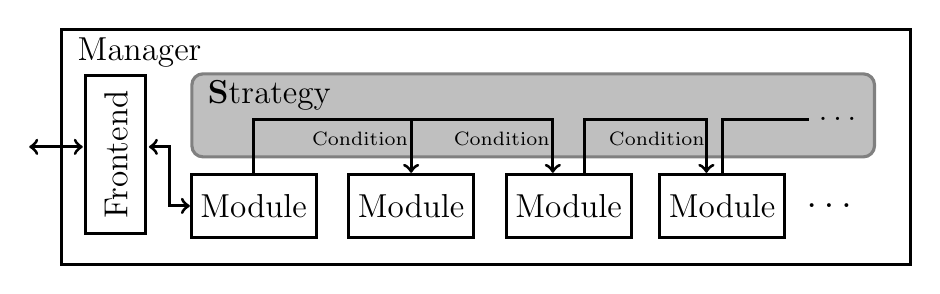
\begin{tikzpicture}[every node/.style={rectangle}, text centered, bend angle=15, line width=.4mm]
	\node[draw, minimum height=57pt, text width=15pt] (manager) at (-6.3, .2) {};
	\node[rotate=90] (managerText) at (-6.3, .2) {\large Frontend};
	\node[draw, minimum height=85pt, text width=300pt] (manager) at (-1.6, 0.3) {};
	\node[] (managerText) at (-6, 1.5) {\large Manager};
	\node[fill=lightgray,draw=gray, rounded corners, minimum height=30pt, text width=240pt] (strategy) at (-1,.7) {};
	\node[] (strategyText) at (-4.35, .95) {\large\textbf Strategy};
	\draw[<->] (-5.36,-.45) -- (-5.62,-.45) -- (-5.62,.3) -- (-5.88,.3);
	\draw[<->] (-6.72,.3) -- (-7.4,.3);
	\draw[->] (-4.55,-.03) -- (-4.55,.65) -- (-.75,.65) -- (-.75,-.03);
	\node[] (strategyText) at (-1.4, .4) {\scriptsize Condition};
	\draw[->] (-2.55,.65) -- (-2.55,-.03);
	\node[] (strategyText) at (-3.2, .4) {\scriptsize Condition};
	\draw[->] (-.35,-.03) -- (-0.35,.65) -- (1.2,.65) -- (1.2,-.03);
	\node[] (strategyText) at (.57, .4) {\scriptsize Condition};
	\draw (1.4,-.03) -- (1.4,.65) -- (2.5,.65);
	\node[] (dotsa) at (2.9,.65) {\large \ldots};
	\node[draw, minimum height=23pt] (moduleAText) at (-4.55, -.45) {\large Module};
	\node[draw, minimum height=23pt] (moduleBText) at (-2.55, -.45) {\large Module};
	\node[draw, minimum height=23pt] (moduleCText) at (-.55, -.45) {\large Module};
	\node[draw, minimum height=23pt] (moduleDText) at (1.4, -.45) {\large Module};
	\node[] (dotsc) at (2.8, -.45) {\Large \ldots};
\end{tikzpicture}%

\end{center}
\label{fig:frameworka}
\end{figure}

\begin{figure}[ht]
\caption{A snapshot of an \smtrat composition being a theory solver embedded in an SMT solver.}
\begin{center}
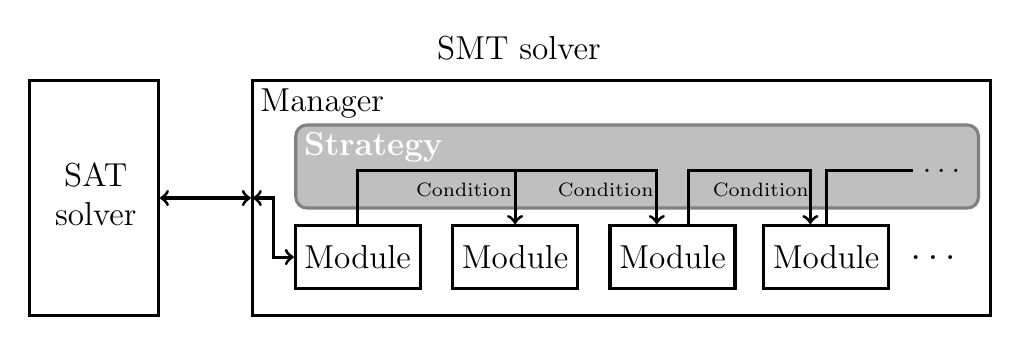
\begin{tikzpicture}[every node/.style={rectangle}, text centered, bend angle=15, scale=1, line width=.4mm]
	\node[] (smtsolver) at (-2.5, 2.2) {\large SMT solver};
	\node[draw, minimum height=85pt, text width=40pt] (satsolver) at (-7.9, 0.3) {\large\begin{tabular}{c}SAT \\ solver\end{tabular}};
	\node[draw, minimum height=85pt, text width=260pt] (manager) at (-1.2, 0.3) {};
	\node[] (managerText) at (-5, 1.5) {\large Manager};
	\node[fill=lightgray,draw=gray, rounded corners, minimum height=30pt, text width=240pt] (strategy) at (-1,.7) {};
	\node[] (strategyText) at (-4.35, .95) {\large\bf \color{white} Strategy};
	\draw[<->] (-5.36,-.45) -- (-5.62,-.45) -- (-5.62,.3) -- (-5.88,.3);
	\draw[->] (-4.55,-.03) -- (-4.55,.65) -- (-.75,.65) -- (-.75,-.03);
	\node[] (strategyText) at (-1.4, .4) {\scriptsize Condition};
	\draw[->] (-2.55,.65) -- (-2.55,-.03);
	\node[] (strategyText) at (-3.2, .4) {\scriptsize Condition};
	\draw[->] (-.35,-.03) -- (-0.35,.65) -- (1.2,.65) -- (1.2,-.03);
	\node[] (strategyText) at (.57, .4) {\scriptsize Condition};
	\draw (1.4,-.03) -- (1.4,.65) -- (2.5,.65);
	\node[] (dotsa) at (2.9,.65) {\large \ldots};
	\node[draw, minimum height=23pt] (moduleAText) at (-4.55, -.45) {\large Module};
	\node[draw, minimum height=23pt] (moduleBText) at (-2.55, -.45) {\large Module};
	\node[draw, minimum height=23pt] (moduleCText) at (-.55, -.45) {\large Module};
	\node[draw, minimum height=23pt] (moduleDText) at (1.4, -.45) {\large Module};
	\node[] (dotsc) at (2.8, -.45) {\Large \ldots};
	\path[<->] (satsolver.0) edge[] node[left] {} (manager.180);
\end{tikzpicture}

\end{center}
\label{fig:frameworkb}
\end{figure}

Based on \carl's data structures and basic functions, a rich set of SMT compliant implementations of \supportedLogics procedures is provided by \smtrat. Each procedure is encapsulated in a \emph{module}, which fixes a common interface, and they can then be composed to a solver according to a user defined \emph{strategy}. A \emph{manager} maintains their allocation to \emph{solving tasks} according to the strategy and provides the API, including the parsing of an \smtlibfile.

\section{Modules}
A module $m$ holds a set of formulas, called its \emph{set of received formulas} and denoted by $\Crcv(m)$. The main function of a module is \texttt{check(bool full)}, which either decides whether $\Crcv(m)$ is satisfiable or not, returning \SAT or \UNSAT, respectively, or returns \UNKNOWN. A set of formulas is semantically defined by their conjunction. If the function's argument \texttt{full} is set to \false, the underlying procedure of $m$ is allowed to omit hard obstacles during solving at the cost of returning \UNKNOWN in more cases. We can manipulate $\Crcv(m)$ by adding (removing) formulas $\varphi$ to (from) it with \texttt{add($\varphi$)} (\texttt{remove($\varphi$)}). Usually, $\Crcv(m)$ is only slightly changed between two consecutive \texttt{check} calls, hence, the solver's performance can be significantly improved if a module works incrementally and supports backtracking. In case $m$ determines the unsatisfiability of $\Crcv(m)$, it has to compute at least one preferably small \emph{infeasible subset} $\Cinf(m)\subseteq \Crcv(m)$. Moreover, a module can specify \emph{lemmas}, which are valid formulas. They encapsulate information which can be extracted from a module's internal state and propagated among other modules. Furthermore, a module itself can ask other modules for the satisfiability of its \emph{set of passed formulas} denoted by $\Cpass(m)$, if it invokes the procedure \texttt{runBackends(bool full)} (controlled by the manager). It thereby delegates work to modules that	 may be more suitable for the problem at hand. 

\section{Strategy}
\label{sec::strategy}
\smtrat allows a user to decide how to compose the modules. For this purpose we provide a graphical user interface, where the user can create a \emph{strategy} specifying this composition. A strategy is a directed tree $T:=(V, E)$ with a set $V$ of modules as nodes and $E\subseteq V\times \Omega\times\Sigma\times V$, with $\Omega$ being the set of \emph{conditions} and $\Sigma$ being the set of \emph{priority values}. A condition is an arbitrary Boolean combination of formula properties, such as propositions about the Boolean structure of the formula, e.g., whether it is in conjunctive normal form (CNF), about the constraints, \eg whether it contains equations, or about the polynomials, e.g., whether they are linear. Furthermore, each edge carries a unique priority value from $\Sigma=\{1,\ \ldots,\ |E|\}$.

\section{Manager}
The \emph{manager} holds the strategy and the SMT solver's input formula $C_{input}$. Initially, the manager calls the method \texttt{check} of the module $m_r$ given by the root of the strategy with $\Crcv(m_r) = C_{input}$. Whenever a module $m\in V$ calls \texttt{runBackends}% for its passed formula $\Cpass(m)$
, the manager adds a \emph{solving task} $(\sigma,\ m,\ m')$ to its priority queue $Q$ of solving tasks (ordered by the priority value), if there exists an edge $(m,\ \omega,\ \sigma,\ m')\in E$  in the strategy such that $\omega$ holds for $\Cpass(m)$. If a processor $p$ on the machine where \smtrat is executed on is available, the first solving task of $Q$ is assigned to $p$ and popped from $Q$. The manager thereby starts the method \texttt{check} of $m'$ with $\Crcv(m') = \Cpass(m)$ and passes the result (including infeasible subsets and lemmas) back to $m$. The module $m$ can now benefit in its solving and reasoning process from this shared information. Note that a strategy-based composition of modules works incrementally and supports backtracking not just within one module but as a whole. This is realized by a mapping in each module $m$ of its passed formulas $\varphi\in\Cpass(m)$ to sets $R_1,\ldots,\ R_n \subseteq \Crcv(m)$ such that each $R_i$ forms a reason why $m$ included $\varphi$ in $\Cpass(m)$ to ask for its satisfiability. In order to exploit the incrementality of the modules, all parallel executed backends terminate in a consistent state (instead of just being killed), if one of them finds an answer.
  
\section{Procedures implemented as modules}
\label{sec:implemented_modules}
The heart of an SMT solver usually forms a SAT solver. In \smtrat, the module \satModule abstracts $\Crcv(\satModule)$ to propositional logic and uses the efficient SAT solver \texttt{minisat}~\cite{minisat} to find a Boolean assignment of the abstraction. It invokes \texttt{runBackends} where $\Cpass(\satModule)$ contains the constraints abstracted by the assigned Boolean variables in a less-lazy fashion~\cite{sebastiani2007lazy}. The module \simplexModule implements the Simplex method equipped with branch-and-bound and cutting-plane procedures as presented in \cite{DM06}. We apply it on the linear constraints of any conjunction of \supportedLogics constraints. For a conjunction of nonlinear constraints \smtrat provides the modules \gbModule, \vsModule and \cadModule, implementing GB~\cite{JLCA_CAI13}, VS~\cite{Article_Corzilius_FCT2011} and CAD~\cite{Article_Loup_TubeCAD} procedures, respectively. Moreover, the module \icpModule uses ICP similar as presented in~\cite{GGIGSC10}, lifting splitting decisions and contraction lemmas to a preceding \satModule and harnessing other modules for nonlinear conjunctions of constraints as backends. The exact procedure is going to be published. The module \cnfModule invokes \texttt{runBackends} on $\Cpass(\cnfModule)$ being the CNF of $\Crcv(\cnfModule)$, and the module \ppModule performs some preprocessing based on factorizations and sum-of-square decompositions of polynomials.

\section{Infeasible subsets and lemmas}
\label{sec::infsubset_lemmas}
Infeasible subsets and lemmas, which contain only formulas from 
$\Cpass(\SATM)$, prune the Boolean search space and hence the number of theory calls. 
Smaller infeasible subsets are usually more advantageous, because they make larger cuts 
in the search space. Lemmas containing new constraints we call
\emph{inventive lemmas} (\emph{non-inventive} otherwise). They might enlarge the 
Boolean search space, but they can reduce the complexity of later theory calls.
When using inventive lemmas, it is important to ensure that the set possible
constraints introduced in such lemmas is finite for a given module and a given 
input formula. Otherwise, the termination of this procedure can not be guaranteed.



\chapter{Constructing an \SmtratLogic formula}
\label{chapter:constructingaformula}
The class \formulaClass represents arbitrary \SmtratLogic formulas, which are
defined according to the following abstract grammar

\[
\begin{array}{rccccccccccccc}
  p &\quad ::=\quad & a & | & b & | & x & | & (p + p) & | & (p \cdot p) & | & (p^e) \\
  v &\quad ::=\quad & u & | & x \\
  s &\quad ::=\quad & f(v,\ldots,v) & | & u & | & x \\
  e &\quad ::=\quad & s = s \\
  c &\quad ::=\quad & p = 0 & | & p < 0 & | & p \leq 0 & | & p > 0 & | & p \geq 0 & | & p \neq 0 \\
 \varphi &\quad ::=\quad & c & | & (\neg \varphi) & | &
 (\varphi\land\varphi) & | &
 (\varphi\lor\varphi) & | & 
 (\varphi\rightarrow\varphi) & | \\ &&
 (\varphi\leftrightarrow\varphi) & | &
 (\varphi\oplus\varphi)
\end{array}
\]

where $a$ is a rational number, $e$ is a natural number greater one, $b$ is a \emph{Boolean variable} and the \emph{arithmetic variable} $x$ is an inherently existential quantified and either real- or integer-valued. We call $p$ a \emph{polynomial} and use a \carl multivariate polynomial with \cln rationals as coefficients to represent it. The \emph{uninterpreted function} $f$ is of a certain \emph{order} $o(f)$ and each of its $o(f)$ arguments are either an arithmetic variable or an \emph{uninterpreted variable} $u$, which is also inherently existential quantified, but has no domain specified. Than an \emph{uninterpreted equation} $e$ has either an uninterpreted function, an uninterpreted variable or an arithmetic variable as left-hand respectively right-hand side. A \emph{constraint} $c$ compares a polynomial to zero, using a \emph{relation symbol}. Furthermore, we keep constraints in a normalized representation to be able to differ them better.

\subsection{Normalized constraints}
A normalized constraint has the form
\[a_1\overbrace{x_{1,1}^{e_{1,1}}\cdot\ldots\cdot x_{1,k_1}^{e_{1,k_1}}}^{m_1}+\ldots+a_n\overbrace{x_{n,1}^{e_{n,1}}\cdot\ldots\cdot x_{n,k_n}^{e_{n,k_n}}}^{m_n}\ + \ d\ \sim \ 0\]
with $n\geq0$, the \emph{$i$th coefficient} $a_i$ being an integral number ($\neq 0$), $d$ being a integral number, $x_{i,j_i}$ being a real- or integer-valued variable and $e_{i,j_i}$ being a natural number greater zero (for all $1\leq i\leq n$ and $1\leq j_i\leq k_i$). Furthermore, it holds that
$x_{i,j_i}\neq x_{i,l_i}$ if $j_i\neq l_i$ (for all $1\leq i\leq n$ and $1\leq j_i, l_i\leq k_i$) and $m_{i_1}\neq m_{i_2}$ if $i_1\neq i_2$ (for all $1\leq i_1,i_2\leq n$). If $n$ is $0$ then $d$ is $0$ and $\sim$ is either $=$ or $<$. In the former case we have the normalized representation of any variable-free consistent constraint, which semantically equals \true, and in the latter case we have the normalized representation of any variable-free inconsistent constraint, which semantically equals \false. Note that the monomials and the variables in them are ordered according the \polynomialOrder of \carl.
Moreover, the first coefficient of a normalized constraint (with respect to this order) is always positive and the greatest common divisor of $a_1,\ldots,\ a_n,\ d$ is $1$. If all variable are integer valued the constraint is further simplified to
\[\frac{a_1}{g}\cdot m_1\ +\ \ldots\ +\ \frac{a_n}{g}\cdot m_n\ + \ d'\  \sim \ 0,\]
where $g$ is the greatest common divisor of $a_1,\ldots,\ a_n$, 
\[\sim'=\left\{
\begin{array}{ll}
\leq, &\text{ if }\sim\text{ is }< \\
\geq, &\text{ if }\sim\text{ is }> \\
\sim, &\text{ otherwise }
\end{array}
\right.\]
and
\[
d' = \left\{
\begin{array}{ll}
\lceil\frac{d}{g}\rceil &\text{ if }\sim'\text{ is }\leq \\[1.5ex]
\lfloor\frac{d}{g}\rfloor &\text{ if }\sim'\text{ is }\geq \\[1.5ex]
\frac{d}{g} &\text{ otherwise }
\end{array}
\right.\]
If additionally $\frac{d}{g}$ is not integral and $\sim'$ is $=$, the constraint is simplified $0<0$, or if $\sim'$ is $\neq$,
the constraint is simplified $0=0$.

We do some further simplifactions, such as the elimination of multiple roots of the left-hand sides in equations and inequalities with the relation symbol $\neq$, e.g., $x^3=0$ is simplified to $x=0$. We also simplify constraints whose left-hand sides are obviously positive (semi)/negative (semi) definite, e.g., $x^2\leq 0$ is simplified to $x^2=0$, which again can be simplified to $x=0$ according to the first simplification rule.

\subsection{Boolean combinations of constraints and Boolean variables}
A formula is stored as a directed acyclic graph, where the intermediate nodes represent the Boolean operations on the sub-formulas represented by the successors of this node. The leaves (nodes without successor) contain either a Boolean variable, a constraint or an uninterpreted equality. Note that equal formulas, that is formulas being leaves and containing the same element or formulas representing the same operation on the same sub-formulas are stored once and are therefore physically the same objects.

The construction of formulas, which are represented by the \formulaClass, is mainly based on the presented abstract grammar. A formula being a leave wraps the objects the corresponding objects representing a Boolean variable, a constraint or an uninterpreted equality, unless for constraints actually a pointer to a constraint is stored. A Boolean combinations of Boolean variables, constraints and uninterpreted equalities consists of a Boolean operator and the sub-formulas it interconnects. For this purpose we firstly create a set of formulas containing all sub-formulas and then construct the Formula. Note that formulas, constraints and uninterpreted equalities are non-mutable, once they are constructed. (TODO: explain mutable member of formulas for information storage) 

We give a small example constructing the formula \[(\neg b\ \land\ x^2-y<0\ \land\ 4x+y-8y^2=0 )\ \rightarrow\ (\neg(x^2-y<0)\ \lor\ b ),\] with the Boolean variable $b$ and the real-valued variables $x$ and $y$, for demonstration. Firstly, we show how to create real and integer valued, Boolean and uninterpreted variables:
\scriptsize
\begin{verbatim}
carl::Variable x = smtrat::newArithmeticVariable( "x", carl::VariableType::VT_REAL );
carl::Variable y = smtrat::newArithmeticVariable( "y", carl::VariableType::VT_REAL );
carl::Variable i = smtrat::newArithmeticVariable( "i", carl::VariableType::VT_INT );
carl::Variable b = smtrat::newBooleanVariable( "b" );
Sort sortS = smtrat::newSort( "S" );
Sort sortT = smtrat::newSort( "T" );
carl::Variable u = smtrat::newUninterpretedVariable( "u", sortS );
carl::Variable v = smtrat::newUninterpretedVariable( "v", sortT );
\end{verbatim}
\normalsize
Next we see an example how to create polynomials, which form the left-hand sides of the constraints:
\scriptsize
\begin{verbatim}
smtrat::Polynomial px( x );
smtrat::Polynomial py( y );
smtrat::Polynomial lhsA = px.pow(2) - py;
smtrat::Polynomial lhsB = smtrat::Rational(4) * px + py - smtrat::Rational(8) * py.pow(7);
\end{verbatim}
\normalsize
Constraints can then be constructed as follows:
\scriptsize
\begin{verbatim}
const smtrat::Constraint* constraintA = smtrat::newConstraint( lhsA, smtrat::Relation::LESS );
const smtrat::Constraint* constraintB = smtrat::newConstraint( lhsB, smtrat::Relation::EQ );
\end{verbatim}
\normalsize
Uninterpreted functions are 
\scriptsize
\begin{verbatim}
const smtrat::Constraint* constraintA = smtrat::newConstraint( lhsA, smtrat::Relation::LESS );
const smtrat::Constraint* constraintB = smtrat::newConstraint( lhsB, smtrat::Relation::EQ );
\end{verbatim}
\normalsize
Now, we can construct the atoms of the Boolean formula
\scriptsize
\begin{verbatim}
const smtrat::Formula* atomA = smtrat::newFormula( constraintA );
const smtrat::Formula* atomB = smtrat::newFormula( constraintB );
const smtrat::Formula* atomC = smtrat::newBoolean( b );
\end{verbatim}
\normalsize
and the formula itself:
\scriptsize
\begin{verbatim}
smtrat::PointerSet<smtrat::Formula> subformulasA;
subformulasA.insert( smtrat::newNegation( atomC ) );
subformulasA.insert( atomA );
subformulasA.insert( atomB );
const smtrat::Formula* phiA = smtrat::newFormula( smtrat::AND, subformulasA );
smtrat::PointerSet<smtrat::Formula> subformulasB;
subformulasB.insert( smtrat::newNegation( atomA ) );
subformulasB.insert( atomC );
const smtrat::Formula* phiC = smtrat::newFormula( smtrat::OR, subformulasB );
const smtrat::Formula* phiE = smtrat::newImplication( phiA, phiC );
\end{verbatim}
\normalsize
Note, that $\land$ and $\lor$ are $n$-ary constructors, $\neg$ is a unary constructor and all the other Boolean operators are binary.



\chapter{Embedding of an \smtrat solver composition}
\label{chapter:embedding}
In this section we show how to embed a solver composed as explained
in Chapter~\ref{chapter:composingats}, \eg using the default strategy
solver \texttt{RatOne}. For instance, we could embed a theory solver composed with \smtrat 
into an SMT solver in order to extend its supported logics by \supportedLogics (or any of its sub-logics) 
or embed an SMT solver composed with \smtrat into a model checker for the verification of the 
satisfiability/unsatisfiability of occurring SMT formulas. In Chapter~\ref{chapter:constructingaformula}
we have seen, how to construct an object representing an SMT formula. Having this formula,
we can add it to the formulas, whose conjunction the solver composed with \smtrat has to check later
for satisfiability. Here we give an overview of all interfaces:
\begin{itemize}
	\item \begin{verbatim}bool inform( const FormulaT& )\end{verbatim}
		Informs the solver about a constraint, wrapped by the given formula. 
		Optimally, the solver should be informed about all constraints,
        which it will receive eventually, before any of them is added as part of a formula with the 
        interface \texttt{add(..)}. The method returns \false if it is easy to decide (for any module used in this solver), whether 
        the constraint itself is inconsistent.
	\item \begin{verbatim}bool add( const FormulaT& )\end{verbatim}
		Adds the given formula to the conjunction of formulas, which will be considered for the next 
        satisfiability check. The method returns \false, if it is easy to decide whether the just added formula is not satisfiable
        in the context of the already added formulas. Note, that only a very superficial and cheap satisfiability check
        is performed and mainly depends on solutions of previous consistency checks. In the most cases this method returns \true,
        but in the case it does not the corresponding infeasible subset(s) can be obtained by
        \texttt{infeasibleSubsets()}.
    \item \begin{verbatim}Answer check( bool )\end{verbatim}
    	This method checks the so far added formulas for satisfiability. If, for instance we extend an SMT solver
	by a theory solver composed with \smtrat, these formulas are only constraints. The answer can either be
    	\True, if satisfiability has been detected, or 
    	\False, if the formulas are not satisfiable, and \Unknown, if the composition
    	cannot give a conclusive answer. If the answer has been \True, we get the model, satisfying the conjunction
	of the given formulas, using \texttt{model()} and, if it has been \False, we can obtain infeasible subsets by
	\texttt{infeasibleSubsets()}.
	If the answer is \Unknown, the composed solver is either incomplete (which highly depends on the strategy
	but for NRA it is actually always possible to define a strategy for a complete \smtrat solver) or it
	communicates lemmas/tautologies, which can be obtained applying \texttt{lemmas()}. 
	If we embed, e.g., a theory solver composed with \smtrat into an
	SMT solver, these lemmas can be used in its sat solving process in the same way as infeasible subsets are 
	used. The strategy of an SMT solver composed with \smtrat has to involve a \satModule before any theory module
	is used\footnote{It is possible to define a strategy using conditions in a way, that we achieve an SMT solver, even if for some cases no \satModule is involved before a theory module is applied.} and, therefore, the SMT solver never communicates these lemmas as they are already processed by the
	\satModule. A better explanation on the modules and the strategy are given in Section~\ref{sec:managerstrategy} 
	of the last chapter and Chapter~\ref{chapter:composingats}. If the Boolean argument of the function \texttt{check} is \false, the composed solver is allowed to omit hard obstacles during solving at the cost of returning \UNKNOWN in more cases.
     \item \begin{verbatim}void push()\end{verbatim}
    	Pushes a backtrack point to the stack of backtrack points.
    \item \begin{verbatim}bool pop()\end{verbatim}
    	Pops a backtrack point from the stack of backtrack points and undoes everything
		which has been done after adding that backtrack point. It returns \false if no backtrack
		point is on the stack. Note, that \smtrat supports incrementality, that means, that by removing
		everything which has been done after adding a backtrack point, we mean, that all 
		intermediate solving results which only depend on the formulas to remove are deleted. It is highly
		recommended not to remove anything, which is going to be added directly afterwards.
    \item \begin{verbatim}const std::vector<FormulasT>& infeasibleSubsets() const\end{verbatim}
    	Returns one or more reasons for the unsatisfiability of the considered conjunction of 
    	formulas of this \smtrat composition. A reason
    	is an infeasible subset of the sub-formulas of this conjunction.
    \item \begin{verbatim}const Model model() const\end{verbatim}
    	Returns an assignment of the variables, which occur in the so far added
        formulas, to values of their domains, such that it satisfies the 
        conjunction of these formulas. Note, that an assignment is only provided if the conjunction of so far added
        formulas is satisfiable. Furthermore, when solving non-linear real arithmetic 
        formulas the assignment could contain other variables or freshly introduced
        variables.
    \item \begin{verbatim}std::vector<FormulaT> lemmas() const\end{verbatim}
    Returns valid formulas for the purposes as explained in Section~\ref{sec::infsubset_lemmas}. Note, 
    that for instance the \icpModule might return lemmas being splitting decisions, which need to be processed in, \eg a SAT solver. A \emph{splitting decision} has in general the form
    \[(c_1 \land \ldots \land c_n)\ \rightarrow (p \leq r\ \lor\ p > r)\]
    where $c_1,\ldots,\ c_n$ are constraints of the set of currently being checked constraints (forming a \emph{premise}), $p$ is a polynomial (in the most cases consisting only of one variable) and $r\in\Q$. Hence, splitting decisions always form a tautology. We recommend to use the \icpModule only in strategies with a preceding \satModule. The same holds for the \simplexModule, \vsModule, and \cadModule if used on NIA formulas. Here, again, splitting decisions might be communicated.
\end{itemize}



\chapter{Implementing further modules}
\label{chapter:implementingamodule}
In this chapter we explain how to implement further modules. A module is a derivation
of the class \texttt{Module} and we give an 
introduction to its members, interfaces and auxiliary methods in the following of this
chapter. A new module and, hence, the corresponding \Cpp source and header files can be easily
created when using the script \texttt{writeModules.py}. Its single argument is the module's name
and the script creates a new folder in \texttt{src/lib/modules/} containing the
source and header file with the interfaces yet to implement. A new module should be created
only this way, as the script takes care of a correct integration of the corresponding code
into \smtrat.

\section{Members of a module}
Here is an overview of those members of the class \texttt{Module}, which can be accessed directly.
They form the most important ones for an implementation of a new module.

\begin{itemize}
	\item \begin{verbatim}vector<set<const Formula*>> mInfeasibleSubsets\end{verbatim}
		Stores the infeasible subsets of the so far received formulas, if the module determined that
		their conjunction is not satisfiable.
	\item \begin{verbatim}Manager* const mpManager\end{verbatim}
		A pointer to the manager which maintains the allocation of modules (including this one) to other 
		modules, when they call a backend for a certain formula. For further details see Chapter~\ref{chapter:composingats}.
	\item \begin{verbatim}Formula* mpReceivedFormula\end{verbatim}
		Stores the conjunction of the so far received formulas, which this module considers
		for a satisfiability check.
	\item \begin{verbatim}Formula* mpPassedFormula\end{verbatim}
		Stores the conjunction of the formulas which this module has passed to a backend to be
		solved for satisfiability.
\end{itemize}

\section{Interfaces to implement}
In the following we explain which interfaces must be implemented in a module.

\subsection{Informing about a constraint}
\begin{figure}[htb]
\label{fig:exa_inform}
\caption{Example showing how to implement the method \texttt{inform}}
\begin{verbatim}
	bool MyModule::inform( const Constraint* const  _constraint )
	{
	    // Write the implementation here.
	}
\end{verbatim}
\end{figure}
Informs the module about the existence of the given constraint usually before
any formula containing constraints is added to this module for consideration
of a later satisfiability check. At least it can be expected, that this method
is called, before a formula containing the given constraint is added 
to this module for consideration of a later satisfiability check. 
Note that this information might be useful for the module, e.g., for the 
initialization of the datastructures it uses.

\subsection{Asserting a received formula}
\begin{figure}[htb]
\label{fig:exa_assertsubformula}
\caption{Example showing how to implement the method \texttt{assertSubformula}}
\begin{verbatim}
	bool MyModule::assertSubformula( Formula::const_iterator _subformula )
	{
	    Module::assertSubformula( _subformula );
	    // Write the implementation here.
	}
\end{verbatim}
\end{figure}
Asserts the formula at the given position in the conjunction of received formulas 
(\texttt{mpReceivedFormula}), meaning that this module has to include this formula
in the next satisfiability check. If the module
can already decide whether the given formula is not satisfiable itself, it returns \false
otherwise \true. In comparison to the interface \texttt{inform}, any previous solving results
could be consulted to determine this information.
Note, that the implementation of a new module might need some initialization in this method
and has always to call \texttt{Module::assertSubformula} at the beginning.

\subsection{Removing a received formula}
\begin{figure}[htb]
\label{fig:exa_removesubformula}
\caption{Example showing how to implement the method \texttt{removeSubformula}}
\begin{verbatim}
	void MyModule::removeSubformula( Formula::iterator _subformula )
	{
	    // Write the implementation here.
	    Module::removeSubformula( _subformula );
	}
\end{verbatim}
\end{figure}
Removes the formula at the given position from the conjunction of received formulas
(\texttt{mpReceivedFormula}). Everything,
which has been stored in this module and depends on this formula must be removed. In the end of
this method, \texttt{Module::removeSubformula} must be called. It handles the removing of everything
depending on this formula in the derived members of this module, including the infeasible subsets,
the passed formula and the mapping of passed formulas to received formulas, which is introduced in
Section~\ref{sec:runbackend}. Hence, you do not need to take care of this.

\subsection{Checking for satisfiability}
\begin{figure}[htb]
\label{fig:exa_check}
\caption{Example showing how to implement the method \texttt{check}}
\begin{verbatim}
	Answer MyModule::check()
	{
	    // Write the implementation here.
	}
\end{verbatim}
\end{figure}
Implements the actual satisfiability check of the conjunction of formulas, which have been asserted in this module.
There are three options how this module can answer: it either determines that the formulas
are satisfiable and returns \true, it determines unsatisfiability and returns
\false, or it cannot give a conclusive answer and returns \texttt{unknown}. Note, that the method \texttt{Answer foundAnswer( Answer )} must
be invoked with the found answer, before return it. Its return value has the same value as its argument and, hence, you could call it the
following (prettying) way:
\begin{verbatim}
Answer MyModule::check()
{
    ...
    return foundAnswer( yourAnswer );
}
\end{verbatim}
Furthermore, modules can always call
a backend in order to check the satisfiability of any conjunction of formulas. How to run the backend is shown in
Section~\ref{sec:runbackend}. A module has also the opportunity to reason about the conflicts
occurred, if it determines unsatisfiability. For this purpose it has store at least one infeasible
subsets of the set of so far received formulas.

\section{Running backend modules}
\label{sec:runbackend}
Modules can always call a backend in order to check the satisfiability of any conjunction of formulas.
Fortunately, there is no need to manage the assertion or removement of formulas to the backend. 
This would be even more involved as we do allow changing the
backend if it is appropiate (more details to this are explained in Chapter~\ref{chapter:composingats}).
Running the backend is done in two steps:
\begin{enumerate}
	\item Change the passed formula to the formula which should be solved by the backend. Keep in mind,
	       that the passed formula could still contain formulas of the previous backend call.
	\item Call \texttt{runBackends()}.
\end{enumerate}
The first step is a bit more tricky, as we need to know which received formulas led to a passed
formula. For this purpose a module contains a mapping from a passed formula to one or more
sets of received formulas. We give a small example by showing the behavior of one of the modules
we provide, the \simplifierModuleClass. Let us assume that this module has so far received the following
constraints:
$$c_0:x\leq0,\ c_1:x\geq 0,\ c_2:x=0$$
\simplifierModuleClass combines the first two constraints $c_0$ and $c_1$ to $c_3:x=0$. Then it combines
$c_3$ with $c_2$ to $c_5:x=0$. Afterwards it calls its backend on the only remaining constraint,
that means the passed constraints contain only $c_5:x=0$. The mapping of $c_5$ to the received constraints it
stems from is $$c_5\ \mapsto\ (\{c_0,\ c_1\},\ \{c_2\}).$$

The mapping is maintained automatically and offers two methods to add formulas to the vector
of the passed formulas:
\begin{itemize}
	\item \begin{verbatim}void addReceivedSubformulaToPassedFormula( Formula::const_iterator )\end{verbatim}
		Adds the formula at the given positition in the conjuntion of the so far received formulas
		to the conjunction of the passed formulas. The mapping to its \emph{original formulas} contains
		only the formula at the given position in the vector of received formula
	\item
		\begin{verbatim}
		void addSubformulaToPassedFormula
		(
		    Formula*,
		    const vec_set_const_pFormula&
		)
		\end{verbatim}
		Adds the given formula to the vector of the passed formulas. It is mapped to the given
		original formulas. Note, that the second argument must contain only subformulas of the conjunction 
		of so far received formulas. We	do not check this by reason of efficiency.
\end{itemize}
If the original formulas of a passed formula are only empty sets, by reason of a belated removing of the according
received formulas, this passed formula will be automatically removed from the backends and the passed formula.

The second step is really just calling \texttt{runBackends()} and processing its return value, which can be
\true, \false, or \texttt{unknown}.

\section{Auxilliary functions}
The \texttt{module} class provides a rich set of methods for debugging purposes. Besides some 
printing methods, \smtrat helps to maintain the correctness of new modules during their development.
It therefore provides methods to store formulas with their assumed satisfiability status in order
to check them belatedly by any SMT solver which is capable to parse \texttt{.smt2} files and solve
the stored formula. To be able to use the following methods, the compiler flag \texttt{SMTRAT\_DEVOPTION\_Validation}
must be activated, which can be easily achieved when using \ccmake.

\begin{itemize}
	\item \begin{verbatim}static void addAssumptionToCheck( const X&, bool, const string& ) \end{verbatim}
		Adds the given formulas to those, which are going to be stored as an \texttt{.smt2} file,
		with the assumption that they are satisfiable, if the given Boolean argument is \true, or unsatisfiable,
		if the given Boolean argument is \false. The formulas can be passed as one of the following types (\texttt{X} can be one of the following datastructures)
		\begin{itemize}
		\item \texttt{Formula} (a single formula of any type)
		\item \texttt{set<const Formula*>} (a set of formulas, which is considered to be a conjunction)
		\item \texttt{set<const Constraint*>} (a set of constraints, which is considered to be a conjunction)
		\end{itemize}
		The third argument of this function is any string which helps to identify the assumption, e.g.,
		involving the name of the module and for which purpose this assumption has been made.
	\item \begin{verbatim}static void storeAssumptionsToCheck( const Manager& )\end{verbatim}
		This method stores all collected assumptions to the file \texttt{assumptions.smt2}, which can be checked
		later by any SMT solver which is capable to parse \texttt{.smt2} files and solve
		the stored formula. As this method is static, we need to pass the module's manager (\texttt{*mpManager}).
		Note that this method will be automatically called when destructing the given manager. Invoking this
		method is only reasonable, if the solving aborts directly afterwards and, hence, omits the manager's
		destructor.
	\item \begin{verbatim}void checkInfSubsetForMinimality
(
    vector<set<const Formula*>>::const_iterator,
    const string&,
    unsigned
) const 
\end{verbatim}
This method checks the infeasible subset at the given position for minimality, that is it checks whether there is a subset of it having maximally $n$ elements less, which is still infeasible.
As for some approaches it is computationally to hard to provide always a minimal infeasible subset, they rather provide infeasible subsets not necessarily being minimal. This method helps 
to ananlyze how close the size of the encountered infeasible subsets is to a minimal one.
\end{itemize}



\chapter{Composing a solver}
\label{chapter:composingats}
\smtrat contributes a toolbox for composing an SMT compliant solver for its supported logics, that means it is incremental, supports backtracking and provides reasons for inconsistency. The resulting
solver is either a fully operative SMT solver, which can be applied
directly on \texttt{.smt2}-files, or a theory solver, which can be embedded into an SMT 
solver in order to extend its supported logics by those provided by \smtrat.

We are talking about composition and toolbox, as \smtrat contains implementations
of many different procedures to tackle, \eg \supportedLogics, each of them
embedded in a module with uniform interfaces. These modules form the tools in the toolbox
and it is dedicated to a user how to use them for solving an SMT formula.
We provide a self-explanatory graphical user interface (GUI) for the definition of a graph-based 
strategy specifying which module(s) should be applied on which formula, 
taking into account the modules which were already involved.

In Section~\ref{sec::strategy} we have already introduced
a strategy and in the following of this chapter we firstly give a brief introduction 
to the existing modules equipped with an estimation of their input-based performances and then illustrate
how to use the GUI for composing a strategy.

\section{Existing module implementation}
\subsection{The \cnferModuleClass}
Transforms its received formula into conjunctive normal form CNF.

\paragraph{Efficiency} The worst case complexity of this module is polynomial in the number of operators in the formula to transform.

\subsection{The \satModuleClass}
This module abstracts it's received formula, being any SMT formula of the supported logics of \smtrat, to it's Boolean skeleton. It thereby replaces all constraints in the formula by fresh Boolean variables. The resulting propositional formula is then solved with \minisat~\cite{minisat}, where after each completed decision level the constraints belonging to the assigned Boolean variables are checked for consistency by the backends of this module. In the case of inconsistency, the infeasible subsets of the backends are abstracted and then involved in the search for a satisfying solution.

\paragraph{Efficiency} Even though the worst case complexity of this procedure, not considering the complexity of the backend calls, is exponential in the number of variables in the abstracted formula, the procedure is in practice more efficient than any of the theory modules. Hence, it does clearly not form a bottleneck of the SMT solving. However, one should aim at reducing the number and complexity of the theory (backend) calls of this module, which might be influenced by infeasible subsets, which are small and/or involve constraints of earlier decision levels in the SAT solving, and lemmas, which either prune the search space of the SAT solving or ease subsequent theory calls.

\subsection{The \lraModuleClass}
Implements the SMT compliant \emph{Simplex} method presented in \cite{DM06}.
Hence, this module can decide the consistency of any conjunction
consisting only of linear real arithmetic constraints. Furthermore,
it might also find the consistency of a conjunction of constraints
even if they are not all linear and calls a backend after removing
some redundant linear constraints, if the linear constraints are satisfiable
and the found solution does not satisfy the non-linear constraints. Note that the 
\lraModuleClass might need to communicate a lemma/tautology to a preceding 
\satModuleClass, if it receives a constraint with the relation symbol $\neq$
 and the strategy needs for this reason to define a \satModuleClass at any 
 position before an \lraModuleClass.

\paragraph{Integer arithmetic} In order to find integer solutions, this
module applies, depending on which settings are used, branch-and-bound,
the construction of Gomory cuts and the generation of cuts from 
proofs~\cite{DilligDA11}. It is also supported to combine these approaches. Note that
for all of them the \lraModuleClass needs to communicate a lemma/tautology to a
preceding \satModuleClass and the strategy needs for this reason to define a 
\satModuleClass at any position before an \lraModuleClass.

\paragraph{Efficiency} The worst case complexity of the implemented
approach is exponential in the number of variables occurring in the
problem to solve. However, in practice, it performs much faster, and
the worst case applies only on very artificial examples. This module
outperforms any module implementing a method that is designed for 
solving formulas with non-linear constraints. If the received formula
contains integer valued variables, the aforementioned methods might not
terminate.
\subsection{The \icpModuleClass}
Implements ..

\paragraph{Efficiency} ..
\subsection{The \gbModuleClass}
Implements the Gr\"obner bases based procedure as presented in~\cite{JLCA_CAI13}. In general, this procedure can detect only the unsatisfiability of a conjunction of equations. This module also supports the usage of these equations to further simplify all constraints in the conjunction of constraints forming its input and passes these simplified constraints to its backends. However, it cannot be guaranteed that backends perform better on the simplified constraints than on the constraints before simplification.

\paragraph{Efficiency} The worst case complexity of the underlying procedure is exponential in the number of variables of the input constraints. In the case that the conjunction of constraints to check for satisfiability contains equations, this module can be more efficient than other modules for NRA on finding out inconsistency.
\subsection{The \vsModuleClass}
Implements the \emph{virtual substitution} method for a conjunction of constraints as described in \cite{}. This module supports incremental calls, efficient backtracking and infeasible subset generation. Note, that the infeasible subsets are often very small but not necessarily minimal. The implemented approach is not complete, as it maybe cannot decide the satisfiability of a conjunction containing a constraint, which involves a variable with degree $3$ or more. Note, that even if no constraint of such form occurs in the received formula, this module might not be able to determine the consistency of its received formula, as it could create constraints of this form in its solving process. Nevertheless, the implemented approach is efficient compared to other approaches for non-linear real arithmetic conjunctions, and therefore well-suited to be used for solving conjunctions of non-linear real arithmetic constraints before complete approaches have their try. In combination with a backend, this module tries to solve the given problem and calls the backend on problems with less variables.

\paragraph{Efficiency} The worst case complexity of this approach is exponential in the number of real arithmetic variables occurring in the conjunction to solve. It performs especially good on almost linear instances and slightly prefers problems only containing constraints with the relation symbols $\leq$, $\geq$ and $=$. It is often the case, that even if the conjunction to solve contains many not suited constraints, this module can determine the consistency on the basis of a well suited subset of the constraints in this conjunction.
\subsection{The \cadModuleClass}
This module implements an adapted version of the \emph{cylindrical algebraic decomposition} (CAD) for a conjunction of constraints as described in \cite{Article_Collins_75}.
It extends the original algorithm to be SMT compliant and implements the ideas from \cite{Article_Loup_TubeCAD}.

The CAD method consists of two basic routines: the projection (or elimination) of polynomials and the lifting (or construction) of samples.
The projection transforms a set of polynomials over a set of variables to a new set of polynomials that do not contain some of the variables.
The lifting starts with a sample point of degree $k$ and constructs a sample point of degree $k+1$ using the polynomial sets from the projection.
Both routines work in an incremental fashion: polynomials are only projected if needed and the construction is performed as a depth-first search.

\paragraph{Efficiency} 
The worst case complexity of this algorithm is doubly exponential in the number of variables, the base being the sum of the number of polynomials and the maximum degree of any polynomial.
This is due to an quadratic increase of polynomials in each projection step and a number of possible sample points that grows with the number of polynomials.

The practical performance heavily depends on the number and degree of polynomials created during the elimination.
It benefits greatly if the real roots of the polynomials are rational, as irrational root operation may take quite some time.


\section{Specifying a strategy with the GUI}

The following subsections are used to give an overview of the 
 \smtrat's GUI, which we call \smtxrat, and to introduce its functionalities.

\subsection{Concept}
\label{sec:concept_of_smt-xrat}
The underlying concept of \smtxrat is the user-guided, visual 
modeling of module compositions in form of graphs and their 
mapping onto their corresponding source code for \smtrat. A 
modeled graph expresses an intended strategy graph of the user. 
Both can easily be projected on each other, because the data 
structure of a strategy graph also describes a graph structure, 
as explained in the previous chapter. A mapping considers not 
only the modeled hierarchy of the SMT-RAT modules, but also 
their attributes. Furthermore the GUI complies the constraints 
of these attributes during the modeling process, for example 
priority values are required to be unique.

The GUI does not only support the visual creation of strategy 
graphs and their translation into source code, but also enables 
the user to integrate the translated source code into \smtrat or, 
if necessary, delete it subsequently. The conclusive work only 
involves a recompilation of \smtrat with the desired strategy 
graph instance to obtain a customized SMT solver.

\subsection{Main window structure}
\label{sec:main_window_structure_of_smt-xrat}
The main window structure of the \smtxrat application can be seen 
in Figure \ref{fig:smt-xrat_main_window}. It principally consists 
only of one large pane, which is called \emph{strategy graph pane}. 
This pane embodies the workspace of the user and visualizes the 
composition of SMT-RAT modules, which are currently modeled. Only a
comparatively small area is occupied by a compact menu bar, which 
offers for instance the exportation of a strategy graph into \smtrat.
\begin{figure}
  \begin{center}
    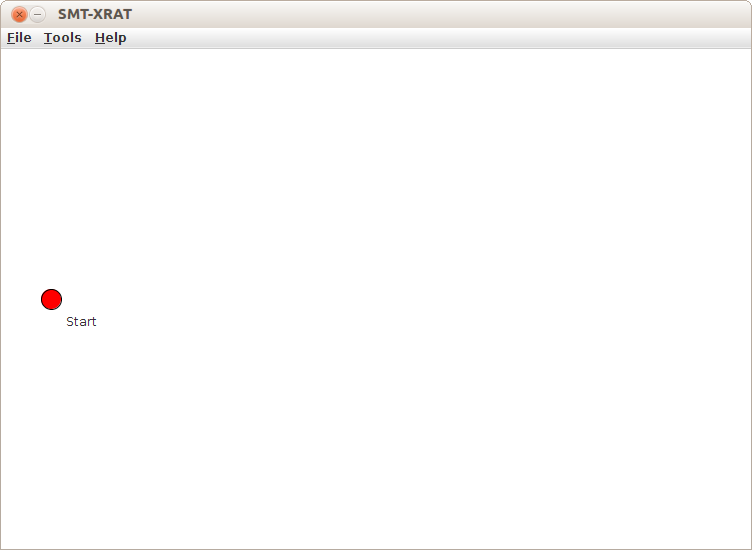
\includegraphics[width=0.9\textwidth]{graphics/smt-xrat_main_window.png}
  \end{center}
  \caption{The main window of the \smtxrat application in its initial state.}
  \label{fig:smt-xrat_main_window}
\end{figure}

\subsection{Strategy graph pane}
\label{sec:the_strategy_graph_pane}
The graphs, which can be modeled in the strategy pane, must be acyclic, directed and weakly 
connected. Nodes represent \smtrat modules and edges represent the call 
hierarchy of them. Both of the element types are labeled to display all 
necessary and editable module attributes within the visualization.
Modeling strategy graphs on the pane implies the interactive operations 
of adding, editing and deleting modules and also aligning elements, 
if desired by the user.

\subsubsection{Adding backends}
\label{sec:adding_backends}
\begin{figure}
  \begin{center}
    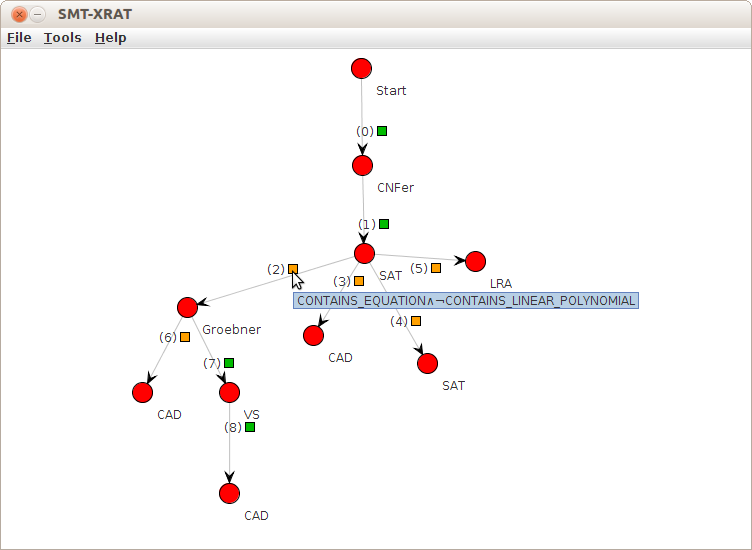
\includegraphics[width=0.9\textwidth]{graphics/smt-xrat_condition_ttt.png}
  \end{center}
  \caption{The small rectangles alongside the edges reveal the hidden condition of a backend.}
  \label{fig:smt-xrat_condition_ttt}
\end{figure}

An initial visualization of the pane contains the inevitable \emph{Start} 
module of an SMT solver, which displays no attributes, but marks the 
starting point for the user to create the desired strategy graph. 
The user can simply consider the \emph{Start} module as the front-end of an 
SMT solver where, \eg \supportedLogics formulas are passed to. Building up a composition of 
modules occurs by appending backends to the \emph{Start} module and then to 
the newly appended backends and so forth. When appending a backend to a 
selected module, a dialog window requests the operating user to input a 
condition and to choose the type of \smtrat module for the new backend. 
The GUI provides a special input interface to enter conditions, which is 
explained later. For each appended backend a new node as well as a directed 
edge from the originating module to this new node is drawn in the visualization. 
In this way, the graph gradually arises on the pane.  A node is labeled with its 
type of \smtrat module whereas an edge holds its condition and an automatically 
assigned priority value. Initially this priority value is always the total number 
of currently existing modules minus $1$, as the \emph{Start} module is not 
counted. As the user-defined conditions might get quite long, they cannot be directly 
seen on the strategy graph pane. Instead, a small rectangle alongside the 
edge reveals them quickly on request. The user needs to point the mouse cursor 
over a rectangle to obtain its corresponding tool tip text, which shows the 
hidden condition, as can be seen in Figure \ref{fig:smt-xrat_condition_ttt}.
This leaves the graph compact and helps to concentrate on the more essential 
aspect of modeling an execution hierarchy. The user can choose to input an 
own condition or leave it by the default value of `\texttt{TRUE}', which, as 
described before, means that given a formula the condition is always satisfied and,
hence, the backends will always be used. 
To point out better which modules contain default conditions and which do not,
the color of a rectangle containing a default condition is green and otherwise 
orange.

\subsubsection{Grammar for conditions}
\label{sec:grammar_for_backend_conditions}
When adding a module to the strategy graph pane, the user has to input a valid
condition for its intended use as backend. A valid condition is a derivation of 
the formal Grammar 
\[{\cal C}=(N, \Sigma, R, S).\] 
The set of nonterminals is given by 
\[N=\{S, T, B, C, D, P\},\] 
whereas the set of terminal symbols 
\[\Sigma=\{\texttt{(}, \texttt{)}, \neg, \leftrightarrow, \oplus, \rightarrow, \land, \lor\} \cup \{\texttt{TRUE}, \texttt{p}_1, \dots, \texttt{p}_n \}\]
consists of the union of logical operators and propositions. $S \in N$ is the 
start symbol of the production rules denoted by the set $R$, which covers the following:
\begin{center}
\begin{tabular}{lccccccccccc}
  $S$ & $\rightarrow$ & \texttt{TRUE} & $|$ & $T$ & $|$ & $C$ & $|$ & $D$ & $|$ & $TBT$ \\
  $T$ & $\rightarrow$ & $P$ & $|$ & $\neg T$ & $|$ & \texttt{(}$C$\texttt{)} & $|$ & \texttt{(}$D$\texttt{)} & $|$ & \texttt{(}$TBT$\texttt{)} \\
  $B$ & $\rightarrow$ & $\leftrightarrow$ & $|$ & $\oplus$ & $|$ & $\rightarrow$ \\
  $C$ & $\rightarrow$ & $C\land C$ & $|$ & $T$ \\
  $D$ & $\rightarrow$ & $D\lor D$ & $|$ & $T$ \\
  $P$ & $\rightarrow$ & $\texttt{p}_1$ & $|$ & \dots & $|$ & $\texttt{p}_n$ \\
\end{tabular}
\end{center}

with the non-terminal symbols $T$ being a term, $B$ being a binary operator, 
$C$ being a conjunction, $D$ being a disjunction and $P$ being a proposition.

The terminal symbols `$\neg$', `$\leftrightarrow$', `$\oplus$', `$\rightarrow$',
`$\land$' and `$\lor$' represent their related logical operators, which, in 
the context of conditions, are negation, equivalence, exclusive or, implication,
conjunction and disjunction respectively. Their semantics is defined as usual.
The terminal symbols `\texttt{(}' and `\texttt{)}' are used, in case several 
different types of logical operators are utilized within one term. They point
out the precedences of the operators in the same way as it is known from 
mathematical contexts. For example, for the term $p_1 \lor p_2 \land p_3$ it 
is unknown, which of the logical operators has the higher precedence. Writing 
the same term with parenthesis as $p_1 \lor (p_2 \land p_3 \texttt{)}$ clarifies, 
that the conjunction operator is of higher precedence.

The propositions $P = \{p_1, \dots, p_n\}$ are as explained in Section~\ref{sec::strategy}. 
This set can vary among releases of the \smtrat, as well as the user can also 
define own propositions. For this reason, the set of propositions is dynamically 
loaded from the \smtrat source code each time the GUI is started. As mentioned in 
the previous chapter, the set of \smtrat modules can vary as well. Therefore the 
list of available \smtrat modules is also dynamically loaded.

\subsubsection{Interface for inputting conditions}
\label{subsec:improved_interface_for_inputting_conditions}
When adding backends to existing modules on the strategy graph pane, a dialog window
requests the user to input a condition, which must be derivable from the 
above defined Grammar $\cal C$. This dialog window is equipped with additional 
features to ease the input process for the user and to improve the usability. 
A specialized text area is used for inputting conditions. Initially, it contains
the default proposition value `\texttt{TRUE}'. The window also contains a combo box, 
where the user has the possibility to choose a proposition value from. A chosen 
proposition value can then be copied to the current caret position of the text area. 
Should the occasion arise that the user selects a part of an entered condition 
beforehand, it is simply overwritten by the chosen proposition value. The user can
only input proposition values by using this combo box. Proposition values cannot
be typed into the text area directly. On the one side, this simply prevents mistyping
and, on the other side, the list of propositions might be changed between releases
of \smtrat, as stated before. In many cases it will not be sufficient to use conditions,
which contain just one single proposition. When requiring a Boolean combination of 
conditions, the above stated logical operators are needed. Although, the 
characters of the operators are generally not present on a keyboard, they can just
be typed into the specialized text area of the dialog window. To type in the 
conjunction operator `$\land$', for instance, the user simply needs to hit the 
key `c' on the keyboard. Instead of the character `c', the character `$\land$' 
will then appear in the text area.

In order to increase the user experience even further, the text area treats the
single characters of an inserted proposition value as a block, which cannot be
entered by the caret of the text area. This means, that if the caret is positioned
directly left of an inputted proposition value and the user navigates the caret to
the right, it will jump to the position directly right of the proposition. The
caret will never appear between the characters of a single proposition value. This
is the analogous case for selecting and deleting proposition values. All characters
of a proposition value are always selected, deselected or deleted at once.

The text area allows to copy and paste conditions or parts of it. Text, which should
be pasted into the text area, is checked to guarantee, that it only contains allowed
values. Otherwise it will be refused. Allowed values cover proposition values, the
characters used to express logical operators and parenthesis.

When the user confirms the dialog window, the implemented recursive descent parser of
\smtxrat checks, whether the inputted condition is a valid derivation of Grammar
$\cal C$ or not. In case it is not, the user will be returned to the dialog window
to re-edit the condition, as can be seen in Figure~\ref{fig:smt-xrat_condition_wrong}.
Otherwise the inputted condition is adopted for the backend.

\begin{figure}
  \begin{center}
    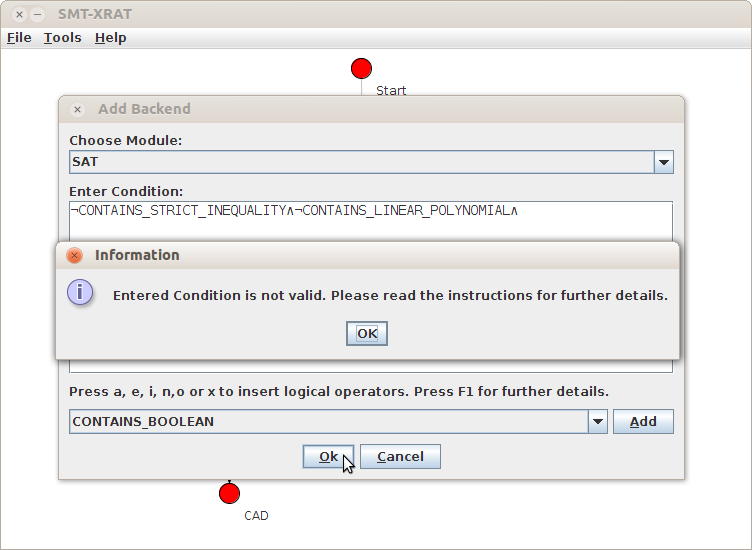
\includegraphics[width=0.9\textwidth]{graphics/smt-xrat_condition_wrong.png}
  \end{center}
  \caption{A wrong condition has been inputted by the user.}
  \label{fig:smt-xrat_condition_wrong}
\end{figure}

\subsubsection{Manipulating the strategy graph}
\label{sec:manipulating_the_strategy_graph}
Besides the capability of adding modules, the strategy graph pane gives the user
also the possibility to remove and edit them subsequently.

The deletion of a single module implicates that all of its succeeding modules in
the composition hierarchy will be removed as well. The strategy graph pane is only
allowed to contain one weakly connected graph. Furthermore, when deleting
one or implicitly more modules, the priority values of all remaining modules might
automatically be adjusted to comply the constraints of the priority values (the priority
value of an edge is always greater than the priority values of its preceding edges).
However, the logical priority order remains untouched.

When editing modules, the same dialog window is displayed as for adding modules.
The window components are already filled in with the attributes of the corresponding
module. However, priority values are not manipulated via this dialog window. As said before,
priority values are automatically assigned, when a module is created, and they are 
displayed alongside the edges. The user can manually change the priority order by 
pushing the priority value of a lower prioritized module in front of the priority
value of a higher prioritized one. The user achieves this by using the mouse pointer
to draw a dashed arrow from the edge label of that lower prioritized module to the
edge label of the higher prioritized module, as it is illustrated by Figure~\ref{fig:smt-xrat_priority_a}. Afterwards the lower prioritized module will have a higher
priority than the other one. The priority values of the modules might just be swapped.
If this is not possible, the priority values of the modules and of their preceding modules
are adjusted automatically, so that as a result, the newly prioritized module will be
ordered logically before the other one. The adaptation of the priority values is
emphasized by Figure~\ref{fig:smt-xrat_priority_b}.
\begin{figure}
  \begin{center}
    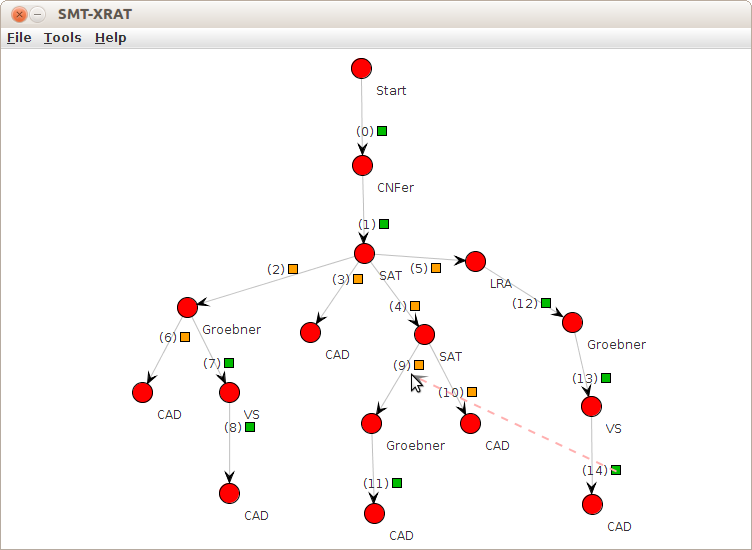
\includegraphics[width=0.9\textwidth]{graphics/smt-xrat_priority_a.png}
  \end{center}
  \caption{Priority values before changes are set.}
  \label{fig:smt-xrat_priority_a}
\end{figure}

\begin{figure}
  \begin{center}
    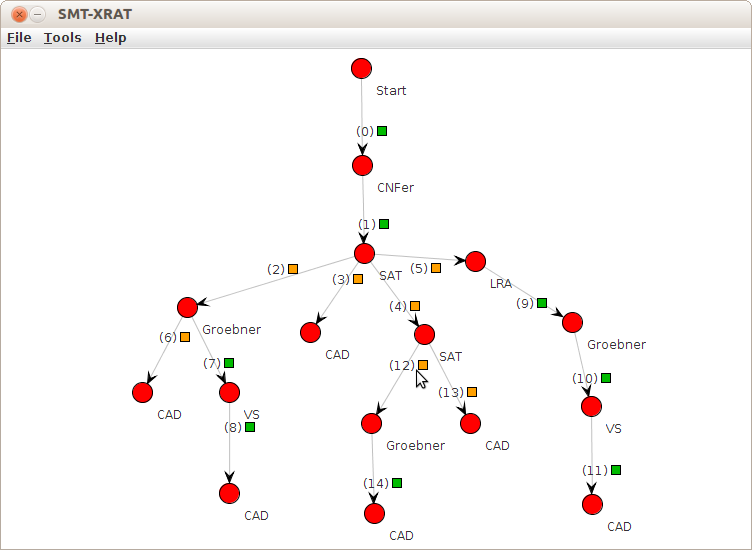
\includegraphics[width=0.9\textwidth]{graphics/smt-xrat_priority_b.png}
  \end{center}
  \caption{Intentionally changed and automatically adapted priority values.}
  \label{fig:smt-xrat_priority_b}
\end{figure}

\subsection{Further functionalities}
\label{sec:further_functionalities}
Further features of the GUI are reached through the menu bar. The most important
and also necessary functionality is the management of strategy graphs inside
the \smtrat source code, \eg the translation of a strategy in the GUI into source code
of \smtrat. To export a currently modeled strategy graph, the user simply needs 
to open the corresponding dialog window and choose a name. Figure~\ref{fig:managing_smt_solvers}
shows an example for exporting the current strategy graph and naming it 
\smtxrat. The GUI will then fulfill the translation and integration process. 
The same dialog window also lists all existing strategy graphs, which are currently 
integrated in the source code, and gives the opportunity to delete them separately.
This can be seen for the existing strategy graph \emph{NRATSolver} of the example.

The remaining features hold by the menu bar are not mandatory, but improve the creation 
process and usability. For example, the GUI allows the user to save the current strategy
graph into an XML file. This file can then be opened again for later editing or it can be
exchanged with another user. Another practical feature is the ability to save a screen shot
of the strategy graph pane into an image file. Such image files can be used to discuss
strategy graphs, when it is not desired to run the GUI.
\begin{figure}
  \begin{center}
    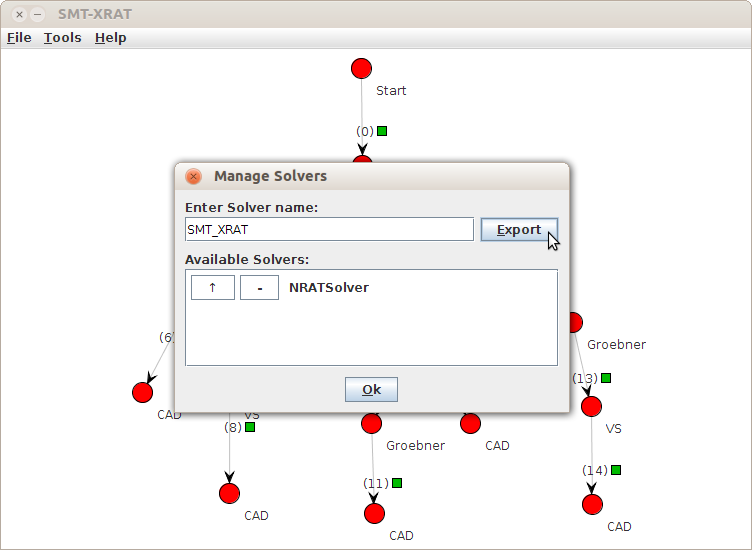
\includegraphics[width=0.9\textwidth]{graphics/smt-xrat_manage_solvers.png}
  \end{center}
  \caption{Managing SMT solvers in the SMT-RAT source code.}
  \label{fig:managing_smt_solvers}
\end{figure}




\chapter{Further features}
\label{chapter:further_features}

\section{Delta debugging}
\emph{Delta debugging} describes a generic debugging approach based on automated testing.
Given a program and an input that provokes a certain behaviour -- for example an error -- delta debugging is the process of iteratively changing the input, retaining the specific behaviour.
Each small change to the input represents a \emph{delta} the name refers to and is the result of some \emph{transformation rule}.
Whenever a change was successful, the change is stored and the process continues from this new changed input.
Eventually, there is no transformation left, such that the faulty behaviour is retained and the debugging process terminates.

This approach only works, if the transformation rules can neither be chained to form a loop, nor continue infinitely.
Usually, as the ultimate goal is a minimal example that triggers some bug, all transformation rules are designed to make the input \emph{smaller}, in one way or another.

As this approach has proven to be very valuable in the context of SMT solving, but existing delta debugging tools\cite{Niemetz2013ddsmt} seemed to be suboptimal to us, SMT-RAT provides its own delta debugging tool \texttt{delta} which can be used completely independent of SMT-RAT.
\texttt{delta} is built to be as generic as possible, but focuses on programs operating on SMTLib files.
It has knowledge of the semantics or logics, but only operates on nodes. Any SMTLib construct, that is either a constant or a braced expression, is a node.

The actual transformation rules are implemented in \texttt{operations.h} and are enabled in the constructor of the \texttt{Producer} class.
The implemented rules are rather simple: removing a node, replacing a node by a child node, simplifying a number, replacing a symbol by a constant or eliminating a let expression.
These transformations are designed such that they can be extended easily.
For a given input \texttt{delta} applies each transformation to each node.
Each application may product arbitrarily many \emph{candidate inputs}, that are then tested. The first candidate that provokes the error is then adopted, the other candidates are rejected.

When analyzing the behaviour, \texttt{delta} relies on the exit code of the program.
It will run the program on the original input and obtain the \emph{original exit code}.
Whenever the program returns the same exit code, \texttt{delta} assumes that the program behaved the same.
Hence, if you want to debug a specific assertion (or error, faulty output, ...), make sure that this event results in a unique exit code.

Using \texttt{delta} is rather easy.
It accepts the input file and the solver as its two main arguments: \texttt{./delta -i input.smt2 -s ./solver}.
There are a couple of other arguments that are documented in the help: \texttt{./delta --help}.


\bibliographystyle{plain}
\bibliography{string,literature,./local,crossref}


\end{document}
